\addtocontents{toc}{\protect\newpage}
\chapter{Differential Equations}
Any equation involving derivatives of a function can be called a differential equation.  For example, $ \dydx=2x$ says ``the derivative equals 2$x$.'' As the derivative of $x^2$, this simple equation also represents a rate-of-change as a function of $x$, or, a differential equation. In this chapter we explore this idea further and look at some mathematical models that take the form of differential equations.

\begin{multicols}{2}
The trajectory of a projectile launched from a cannon follows a curve determined by an ordinary differential equation that is derived from Newton's second law. The relationship between the displacement $x$ and the time $t$ of an object under the force $F$, is given by the differential equation: \[ m\ddxdt=F(x(t)) \]
	 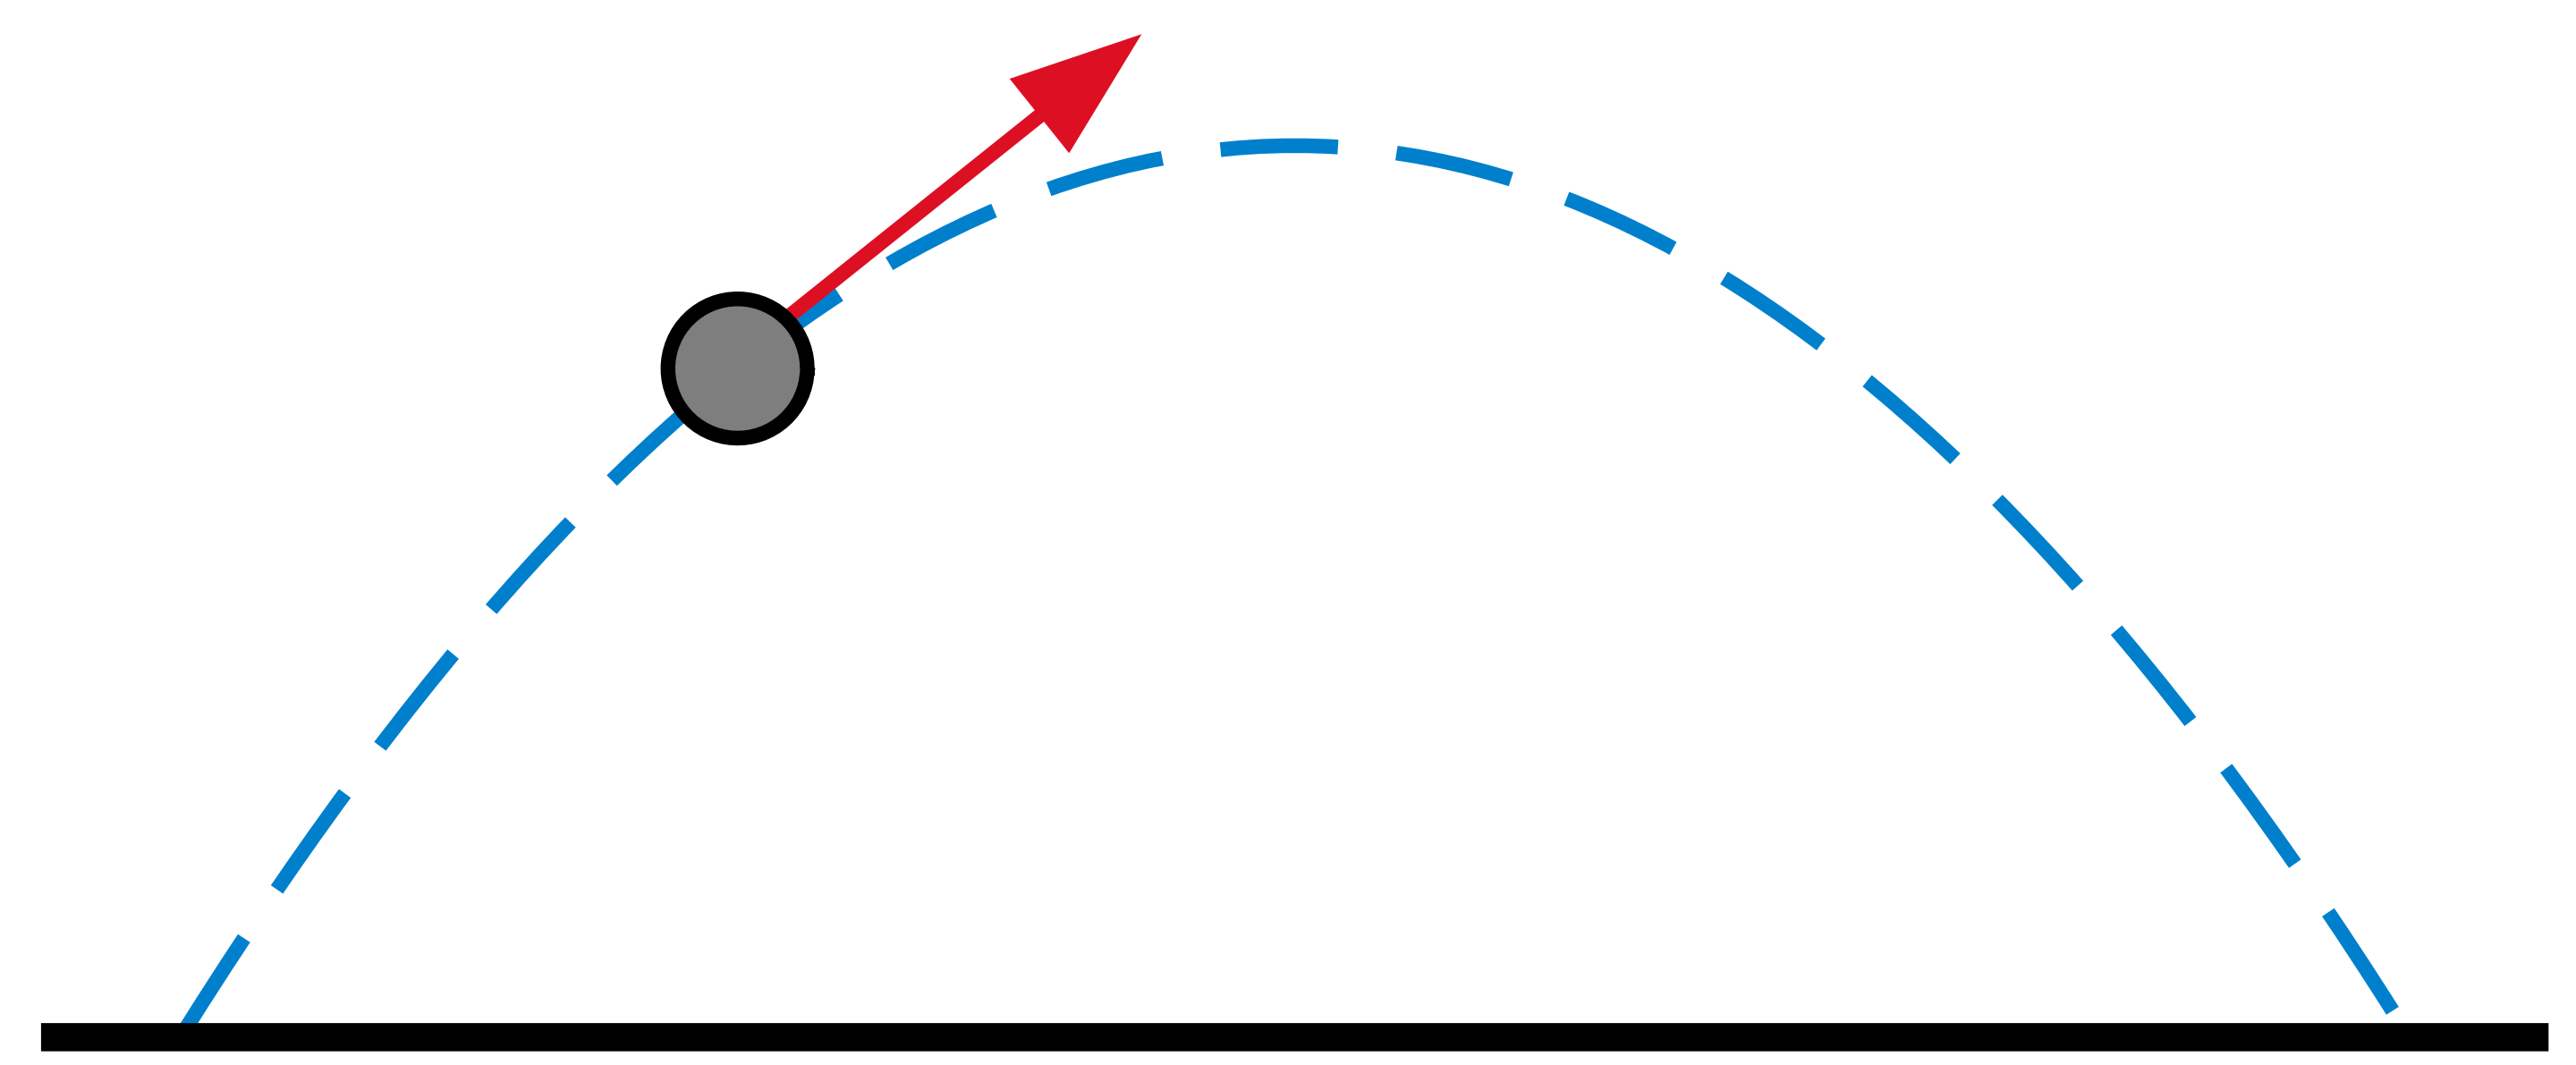
\includegraphics[width=8cm]{DE1}
\end{multicols}
Change is a familiar concept from the slope of the tangent line that we are familiar with. If we have the function, then we can calculate the slope of the tangent at any point on the axis. Now, if the $x$-axis represents time, $t$, this calculation has the possibility of predicting the future! Differential equations can arise when we formulate mathematical models.  We can develop our understanding of this process by considering the mathematical models of some physical phenomena. 



%---------------------------------------------------
% Population Growth
%---------------------------------------------------
\section{Basic Differential Equations}
One model of population growth arises from the assumption that the rate at which the population grows is proportional to the size of the population.
Let $N$ be the size of the population at time $t$ then the rate of change of population with respect to time is $\frac{\mathrm{d} N}{\mathrm{d} t}\text{.}$  So the model can be expressed as a differential equation
\begin{equation*}\frac{\mathrm{d} N}{\mathrm{d} t} =k N
\end{equation*}
where $k$ is the constant of proportionality. 

To make any sense of this model we need to explore the range of values of $N$ and $k$.  $N$ cannot be zero (otherwise there would be nothing to change).  We assume that $N$ is a function of $t$ and that $N (t) >0$.  Similarly for us to have population ``growth''\  $k >0$
\begin{equation*} \therefore \frac{\mathrm{d} N (t)}{\mathrm{d} t} >0
\end{equation*}

We have already shown the properties of the exponential function.  The general exponential function is
\begin{equation*}N (t) =N_{0} e^{k t}
\end{equation*}

Let $N (t)$ be $N_{0}$ when $t =0$.  i.e. $N (0) =N_{0}\text{.}$  $N_{0}$ is called the \emph{initial value} of $N (t)$. 

Now
\begin{align*}\frac{\mathrm{d} N (t)}{\mathrm{d} t} &    = N_{0} e^{k t} \times k \\
 &    = k N (t)\end{align*}

Thus we have shown that $N (t) =N_{0} e^{k t}$ is a solution of the differential equation $\frac{\mathrm{d} N (t)}{\mathrm{d} t} =k N (t)$ 

This solution arises because we are familiar with the behaviour of the exponential function.  Our ability to ``guess''\ the answer is limited so the subject of differential equations involves developing techniques to handle physical situations that are more and more realistic and more and more complex.  The answer to this problem came so simply to us we have to wonder if there are other equations for $N (t)$ that give the same answer. 

%---------------------------------------------------
% The Order of a Differential Equation
%---------------------------------------------------
\section*{The Order of a Differential Equation}
The differential equation $\frac{\mathrm{d} N (t)}{\mathrm{d} t} =k N (t)$ is referred to as a first order differential equation because the order of the highest derivative is \emph{one}.

Here is an example of a second order differential equation
\begin{equation*}m \ddxdt= -k x\end{equation*}

This is the differential equation that arises from Hooke's Law. The second derivative is written $\ddxdt$. Another application from mechanics is found in construction.
\begin{multicols}{2} The elastic curve of a beam under a uniform distributed load will be deflected according to:
	\[M=EI\ddydx\]
Where $M$ is the bending moment acting at $O$. $E$ is Young’s modulus of elasticity of the material of the beam, and $I$ is the moment of inertia of the beam section.\\
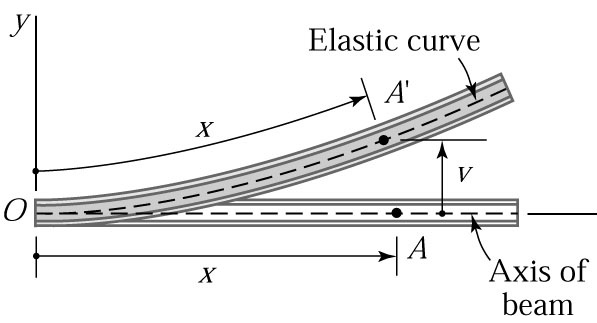
\includegraphics[width=8cm]{DE2}
\end{multicols} 

%---------------------------------------------------
% The Solution of a Differential Equation
%---------------------------------------------------
\section*{The Solution of a Differential Equation}
When you are asked to ``solve''\ a differential equation you are expected to find all possible solutions of the differential equation. Thus, the solution is another function.

\example Find all possible solutions of the differential equation $\dydx =2 x$.  This differential equation could also be expressed as $y^{ \prime } =2 x\text{.}$\medskip\\
\solution By integrating we obtain
\begin{equation*}y =x^{2} +C
\end{equation*}
Where $C$ is the constant of integration.  This is an arbitrary constant and gives us a family of functions all of which are solutions of the differential equation $y^{ \prime } =2 x$.  This family of solutions is often referred to as the \emph{general solution}.

In a physical situation we are often provided with additional information and this will allow us to find a \emph{particular solution}.  This is easy to visualise when considering $y^{ \prime } =2 x\text{.}$  The general solution is $y =x^{2} +C$ and if you are also told that the curve passes through $\left (2 ,6\right )$ you can use this information to evaluate $C\text{.}$
\begin{align*}6 &    = 2^{2} +C \\
C &    = 2\end{align*}

So the particular solution is $y =x^{2} +2$.  To appreciate the concept of this particular solution you only need to use \desmos to
draw $y =x^{2} +C$ for various values of $C$. 

\subsection*{Initial-Value Problems}
In a physical problem when you are given the conditions for the particular solution in the form $y (t_{0}) =y_{0}$ where $t_{0}$ is the initial value of $t$ and $y_{0}$ is the initial value of $y (t)$, the point $\left (t_{0} ,y_{0}\right )$ is called an \emph{initial condition} and the
problem of finding the particular solution given the differential equation is referred to as an \emph{initial-value problem}. 

\example For the differential equation $y^{ \prime } = -y^{2}$ \medskip\\
(a) Verify that $y =\frac{1}{t +C}$ is the general solution \\
(b) Find the solution of the initial-value problem $y^{ \prime } = -y^{2}$ and $y \left (0\right ) =0.5$ \\
%\clearpage
\solution
\begin{tasks}(2)
\task Given $y =\frac{1}{t +C} =\left (t +C\right )^{ -1}$
\begin{align*}y^{ \prime } &    =  -\left (t +C\right )^{ -2} \\
 &    = \frac{ -1}{\left (t +C\right )^{2}} \\
 &    =  -\left(\frac{1}{t +C}\right)^{2} = -y^{2}\end{align*}

So $y =\frac{1}{t +C}$ is the general solution of $y^{ \prime } = -y^{2}$ 

\task Substitute $\left (0 ,0.5\right )$ in $y =\frac{1}{t +C}$
\begin{align*}0.5 &    = \frac{1}{0 +C} \\
\frac{1}{2} &    = \frac{1}{C} \\
C &    = 2\end{align*}
The particular solution is $y =\frac{1}{t +2}$
\end{tasks}
\rule{6.8cm}{0.5pt}\\
\examq\\ Find the particular solution to the differential equation $1+x^2\dydx=x^3$ given that $y(1)=\frac{5}{2}$.\\
\solution Isolate the derivative, $\dydx$, and integrate to find the function $y$:\\
\begin{align*}
\dydx&=\frac{x^3-1}{x^2}\\
\int\dydx&=\int xdx-\int\frac{1}{x^2}dx\\	
y&=\frac{x^2}{2}+\frac{1}{x}+C
\end{align*}
Use the initial condition $y(1)=\frac{5}{2}$ to solve for the unknown constant:\\
	\begin{align*}\frac{5}{2}&=\frac{1^2}{2}+\frac{1}{1}+C\\
	C&=1
	\end{align*}
Therefore the particular solution is $\qquad\displaystyle y=\frac{x^2}{2}+\frac{1}{x}+1$

%---------------------------------------------------
% Separable Equations
%---------------------------------------------------
\section{Separable Equations}
In some special cases we can find explicit solutions of differential equations. One type of equation can be written in the form
\begin{equation*}\dydx =\frac{f (x)}{g (y)}
\end{equation*}

Expressed in this form we simply have to recognise that $f (x)$ is a function without any $y$'s in it and $g (y)$ is a function without any $x$'s in it. The variables can be \textit{separated} by cross-multiplying such that:

\begin{align*}
g (y)\, d y &=f (x)\, d x
\end{align*}
Then we integrate both sides
\begin{equation*}\int g (y) \mathrm{d} y =\int f (x) \mathrm{d} x
\end{equation*}This procedure can be verified by differentiating both sides with respect to $x$
\begin{equation*}\frac{\mathrm{d}}{\mathrm{d} x} \int g (y) \mathrm{d} y =\frac{\mathrm{d}}{\mathrm{d} x} \int f (x) \mathrm{d} x
\end{equation*}By the chain rule the left hand side becomes
\begin{equation*}\frac{\mathrm{d}}{\mathrm{d} y} \int g (y) \,\mathrm{d} y \times \dydx
\end{equation*}So
\begin{align*}\frac{\mathrm{d}}{\mathrm{d} y} \int g (y) \mathrm{d} y \times \dydx &    = \frac{\mathrm{d}}{\mathrm{d} x} \int f (x) \mathrm{d} x \\
g (y) \times \dydx &    = f (x) \\
\text{or\  \  \ }\dydx &    = \frac{f (x)}{g (y)}\end{align*}
\rule{6.8cm}{0.5pt}\\
\example Solve the differential equation by the method of separating variables \[ \dydx =\frac{x^{2}}{y^{2}}\]
\solution The solution to a differential equation is another function. Separate the variables and integrate both sides.
\begin{align*}y^{2} \mathrm{d} y &    = x^{2} \mathrm{d} x \\
\int y^{2} \mathrm{d} y &    = \int x^{2} \mathrm{d} x \\
\frac{y^{3}}{3} &    = \frac{x^{3}}{3} +C \\
y^{3} &    = x^{3} +3 C \\
 &    = x^{3} +C_{1}\end{align*}Where $C_{1}$ is a new arbitrary constant. Isolate $y$ to find a function of the form $y=f(x)$:
\begin{equation*}y =\sqrt[{3}]{x^{3} +C_{1}}
\end{equation*}Find $C_{1}$ given $y (0) =2$
\begin{align*}2 &    = \sqrt[{3}]{0^{3} +C_{1}} \\
C_{1} &    = 8 \\
\text{therefore }y &    = \sqrt[{3}]{x^{3} +8}\end{align*}

\rule{6.8cm}{0.5pt}\\
%\clearpage
\example Solve the differential equation: \[y'=3x^2 y\] 
\solution First write $y^{ \prime } =\dydx$ 
\begin{equation*}\dydx =3 x^{2} y
\end{equation*}Separate the variables
\begin{equation*}\frac{1}{y} \mathrm{d} y =3 x^{2} \mathrm{d} x
\end{equation*}Integrate
\begin{align}\int \frac{1}{y} \mathrm{d} y &    = \int 3 x^{2} \mathrm{d} x \nonumber  \\
\ln  \left \vert y\right \vert  &    = x^{3} +C \tag{1}\end{align}We usually write this by writing in exponential form
\begin{align*}\left \vert y\right \vert  &    = e^{x^{3} +C} \\
 &    = e^{x^{3}} e^{C} \\
y &    =  \pm e^{C} e^{x^{3}}\end{align*}And write $A = \pm e^{C}$ where the value of $A$ is used that satisfies the particular problem
\begin{equation}y =A e^{x^{3}}\tag{2}
\end{equation}

In practice we usually jump from line (1) to line (2) and leave out the intermediate steps. 

%---------------------------------------------------
% Chapter Exercises in a separate file
%---------------------------------------------------
\section{Chapter Exercises}
\subimport{}{6DiffEqnExercises}

